\documentclass[aspectratio=169]{beamer}
\usepackage[english]{babel}
\usepackage{booktabs,listings}
\usepackage[T1]{fontenc}
\usepackage[utf8]{inputenc}


\definecolor{RoboflowPurple}{HTML}{6706CE}
\definecolor{RoboflowGray}{HTML}{4B5563}

\usetheme[slogan=english,mathfont=serif]{NTNU}

	\title[Title]{Embedded AI}
	\subtitle{Real-Time Fastener Detection on Raspberry Pi}
	\author{Bukueva Elena}
	\date{\today}

\begin{document}
	\maketitle
	\begin{frame}{Contents}
		\tableofcontents
	\end{frame}

	\section{Introduction}
	\begin{frame}{A typical slide}
		\begin{itemize}
			\item Write here the introduction
			\item Use \texttt{itemize} or \texttt{enumerate} to organize your main points.
		\end{itemize}
		\begin{block}{Example}
			Rather than freely writing text in the frame, the use of blocks (such as this) is recommended.
			Here you can find a short introduction to the basis of beamer:
			\begin{enumerate}
				\item https://www.overleaf.com/learn/latex/beamer
			\end{enumerate}
		\end{block}
	\end{frame}
    % --- Work Flow ----------------------------------------------
    	\section{Workflow}
	\begin{frame}{Workflow}
		\begin{itemize}
            \item Set up Raspberry Pi 4/5:
                \begin{itemize}
                    \item Install OS
                    \item Connect to the Wi-Fi network
                    \item Install drivers for the camera - IDS SDK
                \end{itemize}
			\item Record videos via the camera, connected to Raspberry Pi
            \item Annotate items via Roboflow framework
            \item Run training on GPU
            \item Test real-time detection on Raspberry Pi
		\end{itemize}
	\end{frame}
    % --- Key camera specs slide ----------------------------------------------
\section{Camera}
\begin{frame}[c]{Camera (UI-3590CP-C-HQ Rev.2)}
  \begin{columns}[c,onlytextwidth]
    \begin{column}[c]{0.58\textwidth}
      \scriptsize\renewcommand{\arraystretch}{1.12}
      \begin{tabular}{@{}ll@{}}
        \toprule
        \multicolumn{2}{l}{\textbf{Sensor}}\\
        \midrule
        Resolution & 18.10 Mpix (4912$\times$3684) \\
        Gain (master/RGB) & 16$\times$ / 4$\times$ \\
        \midrule
        \multicolumn{2}{l}{\textbf{Model}}\\
        \midrule
        Pixel clock range & 96–432\,MHz \\
        Max frame rate (freerun/trigger) & 21 / 21\,fps \\
        Exposure time (min–max) & 0.013–998\,ms \\
        Power consumption & 1.5–3.3\,W \\
        Image memory & 128\,MB \\
        \midrule
        \multicolumn{2}{l}{\textbf{Environment \& I/O}}\\
        \midrule
        Interface & USB 3.0 micro-B, screwable \\
        \bottomrule
      \end{tabular}
    \end{column}

    \begin{column}[c]{0.42\textwidth}
      \centering
      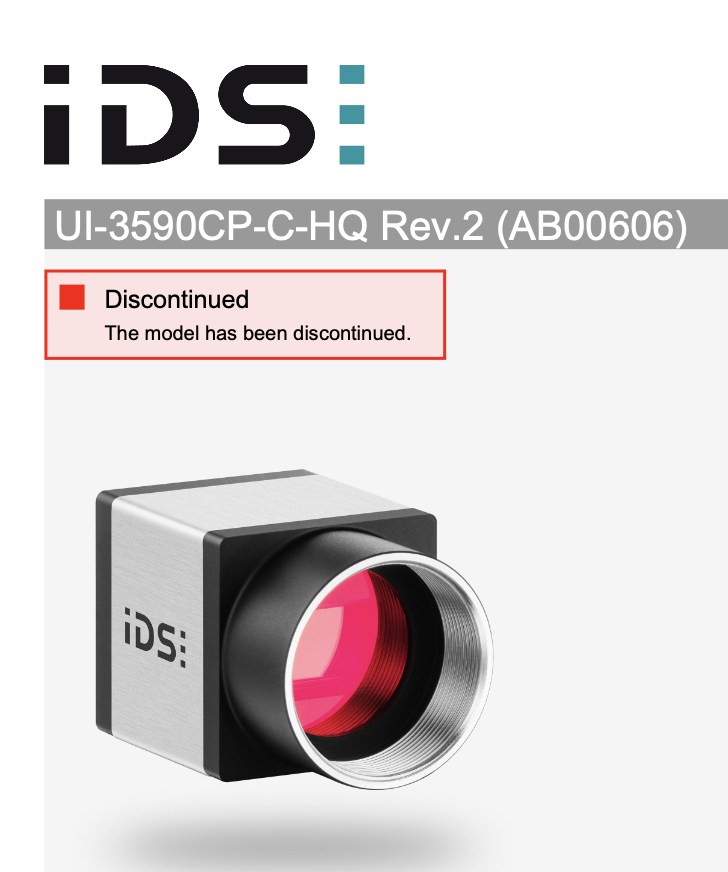
\includegraphics[width=\linewidth]{pics/camera.png}
    \end{column}
  \end{columns}
\end{frame}


    \section{Annotation}
	\begin{frame}{\textcolor{RoboflowPurple}{Roboflow}}
        \vspace{0.6\baselineskip}
        \textcolor{RoboflowGray}{Roboflow is a platform for rapid image annotation, with APIs to upload images
        and export datasets in model-ready formats}
        \vspace{0.4\baselineskip}
        \begin{center}
            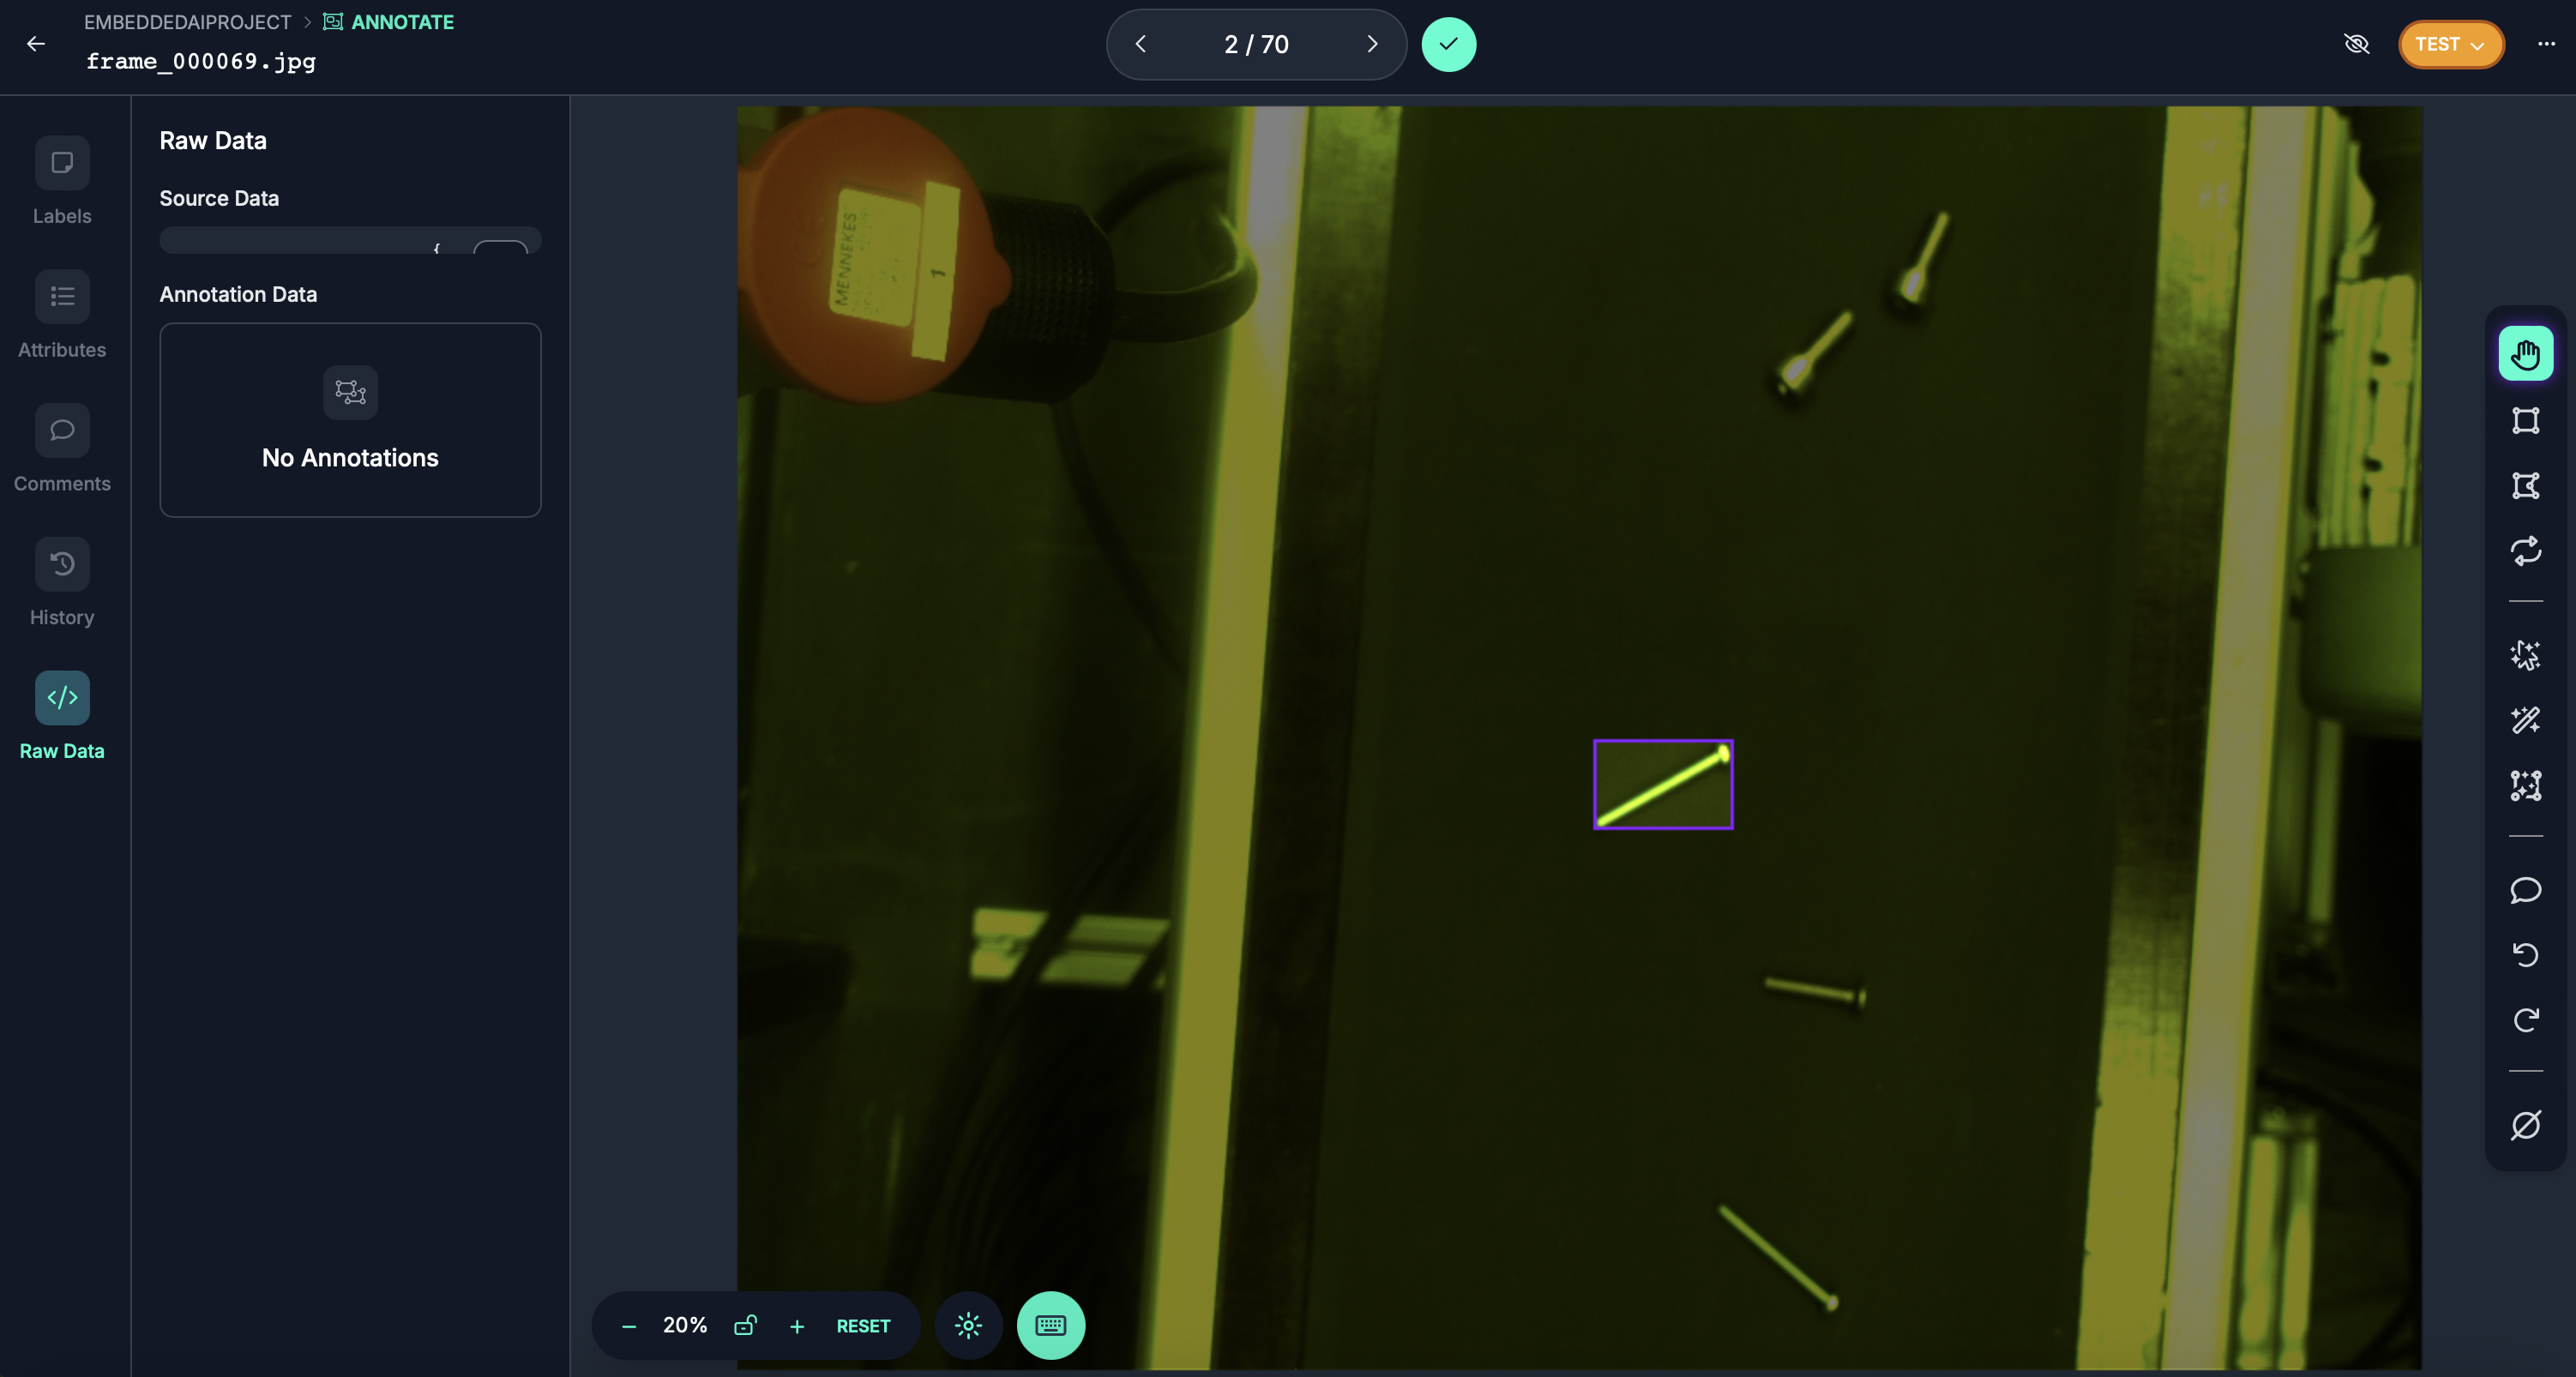
\includegraphics[width=0.7\linewidth]{pics/roboflow_ex.png}
        \end{center}
    \end{frame}

\end{document}
